\section{研究问题与方法定位}
\label{chapter:01}

% block-id: auto.01.p1
\hypertarget{auto.01.p1}{}
科学计算中的一次结果通常经历模型选择、参数解释、软件调用、求解、后处理和论述等环节。这些环节使用不同的数据表示与成功判据：工具能够连接并不说明模型设置正确，求解器正常退出也不说明电流、功率或离散误差满足研究要求。智能体参与建模时，需要把自然语言任务转化为可执行对象，并把每项判断连接到可保存、可检查的证据。

% block-id: auto.01.p2
\hypertarget{auto.01.p2}{}
本研究以 Litz 线为实例，将 Codex 客户端、模型上下文协议 MCP、Wolfram Language 与 Ansys Electronics Desktop 组合为自动化研究流程。Codex 承担任务分解、源码编辑、工具调用和结果解释；MCP 提供工具发现与调用；项目运行器负责输入校验、源码身份、进程资源和产物保存；物理验收由独立计算与明确容差完成。该分工使交互中的探索能够转化为接手者可继续执行的研究对象。\cite{CODEX,MCP,WOLFRAM,AEDT}

% block-id: auto.01.p3
\hypertarget{auto.01.p3}{}
Litz 建模对这一流程提出了具体要求。解析圆线、二维共端模型、有限长度 PEEC、外场 RT0 和三维 A–φ 保留的自由度与激励不同，结果需要按对应观测量解释。换位方法与多尺度建模文献提供了选择模型的基础；逐股复电流、实际铜面积和回流条件则决定不同实现能否直接比较。\cite{P01,N01,RUEHLI1974,RT1977}

% block-id: auto.01.p4
\hypertarget{auto.01.p4}{}
本文研究三个工程问题：如何使客户端、工具和求解器共享可追溯的任务身份；如何把协议检查与物理验收组织成相互衔接的步骤；以及如何在代码扩展、接口错误和数值未通过时保留足够的恢复信息。评价材料来自 rc.2 的六类运行案例，结论对应这些案例实际覆盖的功能。客户端比较、人工操作耗时对照和大样本成功率需要另外设计实验。

% block-id: auto.01.figure
\hypertarget{auto.01.figure}{}
\begin{figure}[!htbp]
\centering
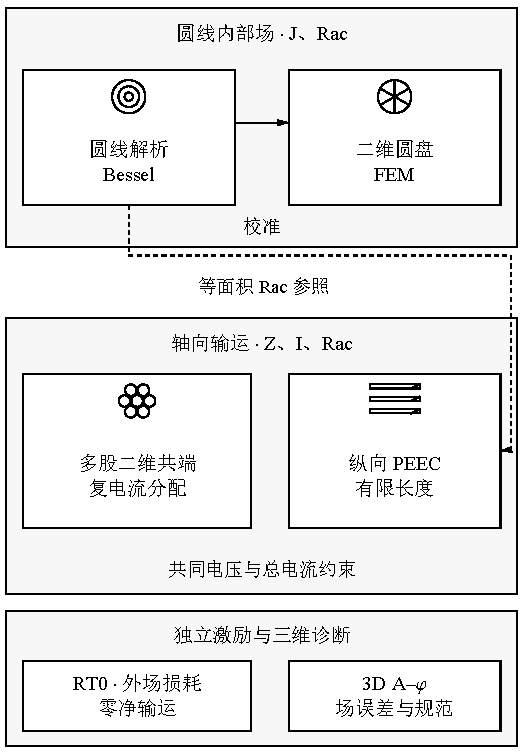
\includegraphics[width=\linewidth,height=.72\textheight,keepaspectratio]{../../assets/zh-CN/model_hierarchy.pdf}
\caption{分层模型与可比较观测量。 输运模型按物理对象与观测量分组：圆线内场用于解析与二维校准，多股二维场路求解共同端口下的复电流，纵向 PEEC 检验有限长度效应。连线标明内部场校准或等面积电阻参照。RT0 外场损耗与三维 A–φ 场诊断各自构成独立研究范围。}
\label{fig:model_hierarchy}
\end{figure}
